% *********************************************************************
% © 2010–2023 Jeremy Sylvestre
%
% Permission is granted to copy, distribute and/or modify this document
% under the terms of the GNU Free Documentation License, Version 1.3 or
% any later version published by the Free Software Foundation; with no
% Invariant Sections, no Front-Cover Texts, and no Back-Cover Texts. A
% copy of the license is included in the appendix entitled “GNU Free
% Documentation License” that appears in the output document of this
% PreTeXt source code. All trademarks™ are the registered® marks of
% their respective owners.
%
% *********************************************************************

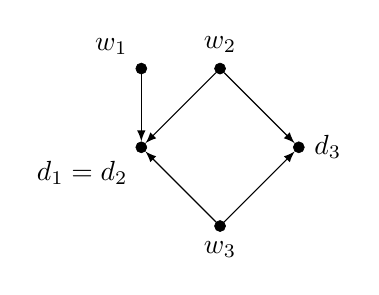
\begin{tikzpicture}[
	vertex/.style={ circle, draw, very thin, fill, inner sep=0pt, minimum size=4pt },
]

\node at (-1,0) (d2) [vertex,label=below left:{$d_1 = d_2$}] {};
\node at (1,0) (d3) [vertex,label=right:{$d_3$}] {};

\node at (-1,1) (w1) [vertex,label=above left:{$w_1$}] {};
\draw[-latex] (w1) to (d2);

\node at (0,1) (w2) [vertex,label=above:{$w_2$}] {};
\node at (0,-1) (w3) [vertex,label=below:{$w_3$}] {};
\foreach \p in {d2,d3} {
	\draw[-latex] (w2) to (\p);
	\draw[-latex] (w3) to (\p);
}

\end{tikzpicture}
